\documentclass[letterpaper, reqno,11pt]{article}
\usepackage[margin=1.0in]{geometry}
\usepackage{color,latexsym,amsmath,amssymb,graphicx, float}
\usepackage{hyperref}

\usepackage[
backend=biber,
sorting=ynt
]{biblatex-chicago}
\addbibresource{sources.bib}

\hypersetup{
colorlinks=true,
linkcolor=magenta,
filecolor=magenta,
urlcolor=cyan,
}
\usepackage{setspace}
\doublespacing

\graphicspath{ {images/} }

\begin{document}
\pagenumbering{arabic}
\title{AMNE 151 Capstone 2\\ \large Option 2: Battle Reimagined}
\date{March 3rd, 2023}
\author{Xander Naumenko, 38198354}
\maketitle

{\bf Fictionalized Account of the Cuban Missile Crisis}

\begin{figure}[htpb]
  \centering
  
\includegraphics[width=0.7\textwidth]{im-athena}
  \caption{My image representation of the account. This was made digitally with Midjourney, an AI image generator. The prompt used was ``Athena as president of the united states in front of an american flag, with a staff in her right hand and a shield in her left.'' It is based off the bronze mirror tracing seen in figure \ref{fig:minerva}. It is meant to symbolize how, just as gods have supreme control over the lives of mortals, political power can assert similar influence.}
  \label{fig:im-athena}
\end{figure}


Athena, president of the United States of America, was the last to enter the meeting room. She took stock of the characters arrayed around the table. On her left were the generals, for the most part maintaining a stoic calmness despite the situation. On her right were the various government officials, diplomats and ambassadors, displaying more nervousness about the real possibility of what they were to discuss today. 

``The Cuban situation must be dealt with.'' Athena stated it not as a query or command, simply as an undeniable truth. ``The united states has rested too long on our laurels of nuclear supremacy, in the comfortable position to be able to fire missiles from Turkey or Italy at our leisure. That era has come to an end. The Soviets have installed missiles in Cuba, and our diplomatic efforts have yet to bear fruit. We are at a turning point of history. Either we accept the communists as our military equals ad infinitum, or we end it all here with our first strike capabilities. I seek your advice here today to settle this matter.''

She sat down in her chair at the head of the table, while the others in the room uncomfortably looked at one another trying to gauge if she was prompting someone specific to speak. After a few moments Robert McNamara, secretary of defense, spoke up. ``Surely you can't be considering a non-retaliatory strike, Ms. President.''

``Of course she is.'' One of the generals responded, after a few seconds had passed and it was clear that Athena was not willing to engage directly in the conversation. ``They have left us with no choice, we have given the ultimatum after ultimatum, and yet they push us still. If we do not respond while we have the militaristic upper hand, how will we fare when we are on equal footing?''

Others hurried to respond, with arguments growing increasingly heated as the evening went on. Athena remained aloof in the discussion, with the full weight of the decision pressing down on her shoulders as she deliberated. After a 3 hours of discussion going around in circles it was clear that everyone in the room, except Athena, had voiced their thoughts. 

``It seems that the time of decision has been reached'' Athena intoned. ``I appreciate the strategic advice you have given me. Of the non nuclear options, it seems that McNamara's plan of naval blockade has the most promise.''

``But that's not enough. I cannot believe in any circumstances that it is a permissible U.S. defensive policy to enable Soviet first strike capabilities. My decision is this: in two days time, we will commence a preemptive nuclear offensive.''

{\bf Explanation of Account}

{\bf Preface note:} {\em In my first capstone in the rubric evaluation I was docked marks for not quoting frequently enough. In both the previous problem statement and the current one it states specifically and unambiguously ``summarize and analyze primary source material rather than quoting it directly.'' I want to follow the problem statement but would not like to be penalized for it, so I'm choosing to follow the requirements of the problem statement by not directly quoting from the texts. Given the strict 300 word limit for 2 primary texts, 2 primary images and one image we make ourselves I don't think it's practical to give quotes for everything in the text. As a compromise I've included direct quotations in footnotes rather than in the text directly. }

The account above is a description of a meeting of top government officials during the Cuban Missile Crisis which, while not a traditional battle, was the closest the Cold War came to nuclear war. Based on the primary texts I believe Athena, faced with such the choice of whether to strike first would decide to be the nuclear aggressor.

One might think that as the more strategic counterpart to Ares, Athena would not rush headlong into terrible battle. However Athena's inherent pride in Ovid's {\em Metamorphoses}\autocite{ovid} are a factor pushing her to horrible deeds. In the text she is jealous of Arachne who has her talents\footnote{After Arachne succeeds in her weaving the text states that ``the golden-haired warrior goddess was grieved by [Arachne's] success.''\parencite{ovid}, line 129}. If she resorts to the violence over something as simple as weaving, it's hard to see her allowing another to gain nuclear supremacy alongside her. Just like Arachne taunts Athena with her depictions of Gods' failings\footnote{Arachne's tapestry is ``embroidered with the gods' crimes,'' \parencite{ovid}, line 130, which to make in front of a goddess was clearly a purposeful affront.}, the Soviet Union's continual small transgressions would very possibly push her over the edge.

The strategic sensibility of a first strike would also appeal to the goddess of wisdom. In Homer's {\em Iliad} book 5\autocite{homer}, she is depicted as levelheaded and strategic, unlike Ares. Whereas Ares massacres ruthlessly, Athena hides with Hade's helm of invisibility to strike at Ares in tandem with Diomedes\footnote{In the text ``Athena donned Hade's helmet of invisibility, to hide her identity from the mighty god.''\parencite{homer}, line 845}. A preemptive strike would cost mortal lives, but in the {\em Iliad} Athena was ordering Greeks to battle and ultimately death over the personal insult of a shepherd, so to Athena it's likely the strategic argument would dominate. 

As for the image aspect required for this capstone, I generated the image seen in figure \ref{fig:im-athena}, and chose the primary source images figures \ref{fig:minerva}\autocite{minerva} and \ref{fig:athena}\autocite{poseidon}. My image generated with Midjourney\autocite{midjourney}\footnote{There doesn't seem to be a standard way to cite AI image generators currently, so I'm currently just leaving the name and website. I spent quite a while trying to find a definitive source with how to do so with no avail. } is intended to show Athena in a modern light with her traditional symbols combined with the American patriotism behind her pushing her to bold decisions. 

\begin{figure}[htpb]
  \centering
  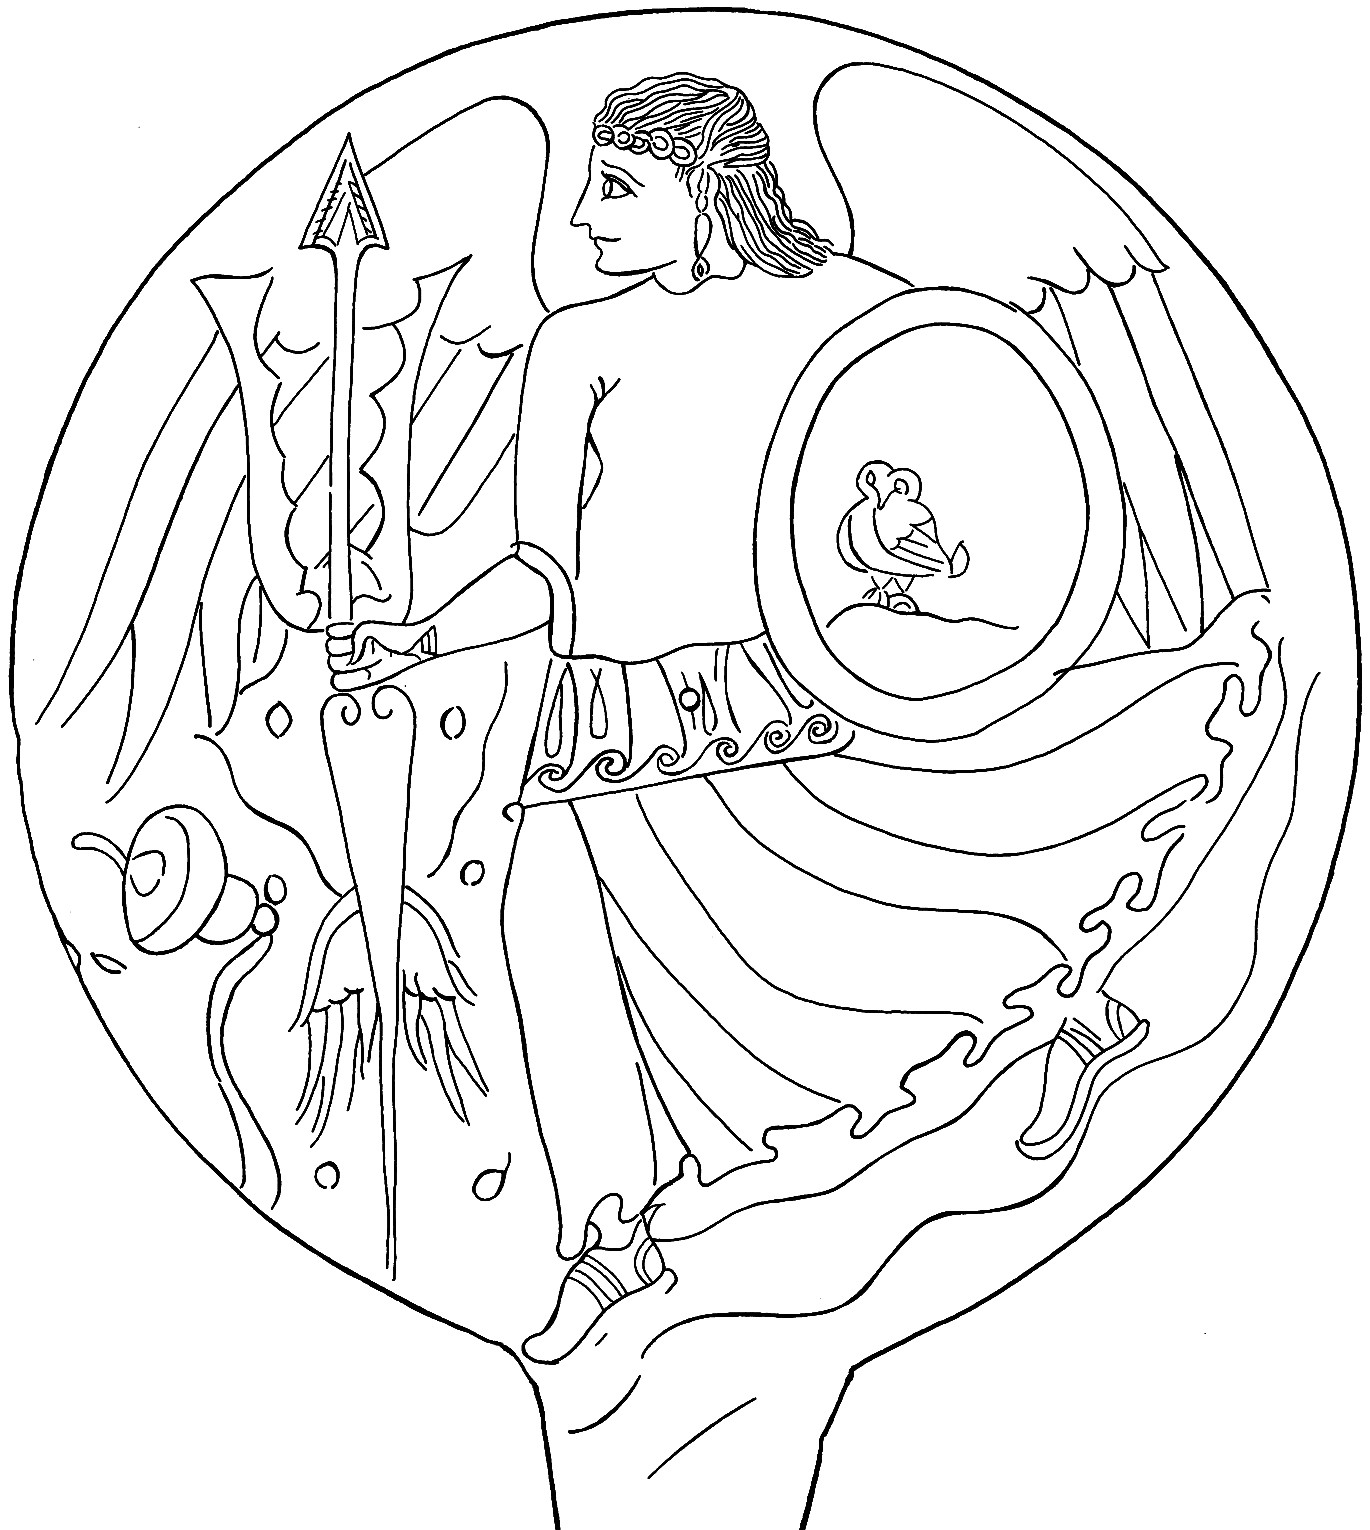
\includegraphics[width=0.5\textwidth]{minerva}
  \caption{\cite{minerva}. An early depiction of what would later become Athena, this is the basis for my generated image seen in figure \ref{fig:im-athena}.}
  \label{fig:minerva}
\end{figure}

\begin{figure}[htpb]
    \centering
    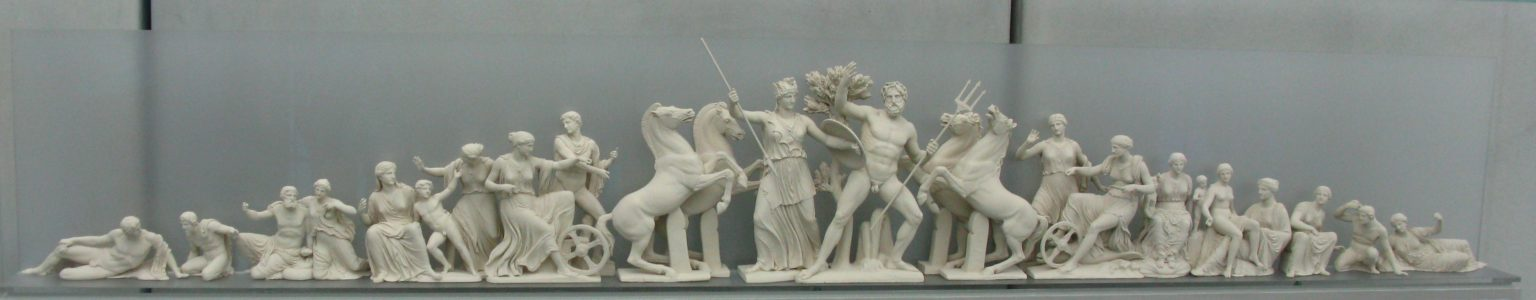
\includegraphics[width=0.8\textwidth]{athena}
    \caption{\cite{poseidon}. A depiction of Athena engaging in a battle of conquest. It seems that the mortals on either side of the gods are suffering from the battle occurring in the middle, but by being depicted as taller it's implied that the Gods' struggles are more relevant. Just like in my account, Athena prioritizes her conquest over the well being of her people.}
    \label{fig:athena}
\end{figure}

\newpage
\newpage
\newpage

\printbibliography

\end{document}
